\documentclass[a4paper,man,biblatex]{apa6}
\usepackage[american]{babel}
\usepackage{csquotes}
\usepackage[backend=biber]{biblatex}
\usepackage[document]{ragged2e}
\setlength{\RaggedRightParindent}{0.5in}
\addbibresource{references.bib}
\usepackage{graphicx}
\usepackage{url}
\usepackage{xpatch}
\xpatchbibdriver{online}
  {\printfield{entrysubtype}}
  {\printfield{entrysubtype}%
   \newunit\newblock
   \printfield{note}}
  {}
  {}

\renewcommand{\abstract}[1]{}

\title{The Rankability of Data}
\shorttitle{The Rankability of Data}
\author{Armant Touche}
\affiliation{Portland State University}
\date{\today}

\begin{document}
\thispagestyle{otherpage}
\setcounter{biburllcpenalty}{7000}
\setcounter{biburlucpenalty}{8000}

%\maketitle

\noindent Name: Armant Touche\newline
\noindent Date: 4/29/2020

\subsection{Description} I wanted to share a research article from the Data Science sphere about a common task that affects everyone of us when we search the Internet. Imagine how Google, Youtube, or other notable online application present search results to us. A lot of you may have heard of "Youtube's algorithm" but the algorithim is an abstract idea that is implemented on other online services other than Youtube. Ranking objects or results requires a lot of questioning. Can we trust the Algorithim? Ranking data is used in applications such as self-driving cars, resource allocation, cybersecurity, and of course, web searches. There are other applications but I wanted to highlight the more common applications we commonly use or are affected by. The figure below is an overview of the relationship between rankability and ranking. Rankability is quantifying a meaningful relationship amongst common objects and objects with high ranking go on to be rank by another process but how rankability is calculated is main topic of this research article because the implication can make or break a online platform. The most common way to represent objects is to used a computer science abstract data structure called graphs. Website like Kayak or Orbitz used this data structure to present the best flights or hotels based off your desired searc. Overall, calculating rankability involves a mix of computer science, lineara algebra, combinatorics, and some other subsets of mathematics which I do not have the tools to describe but just wanted to share.


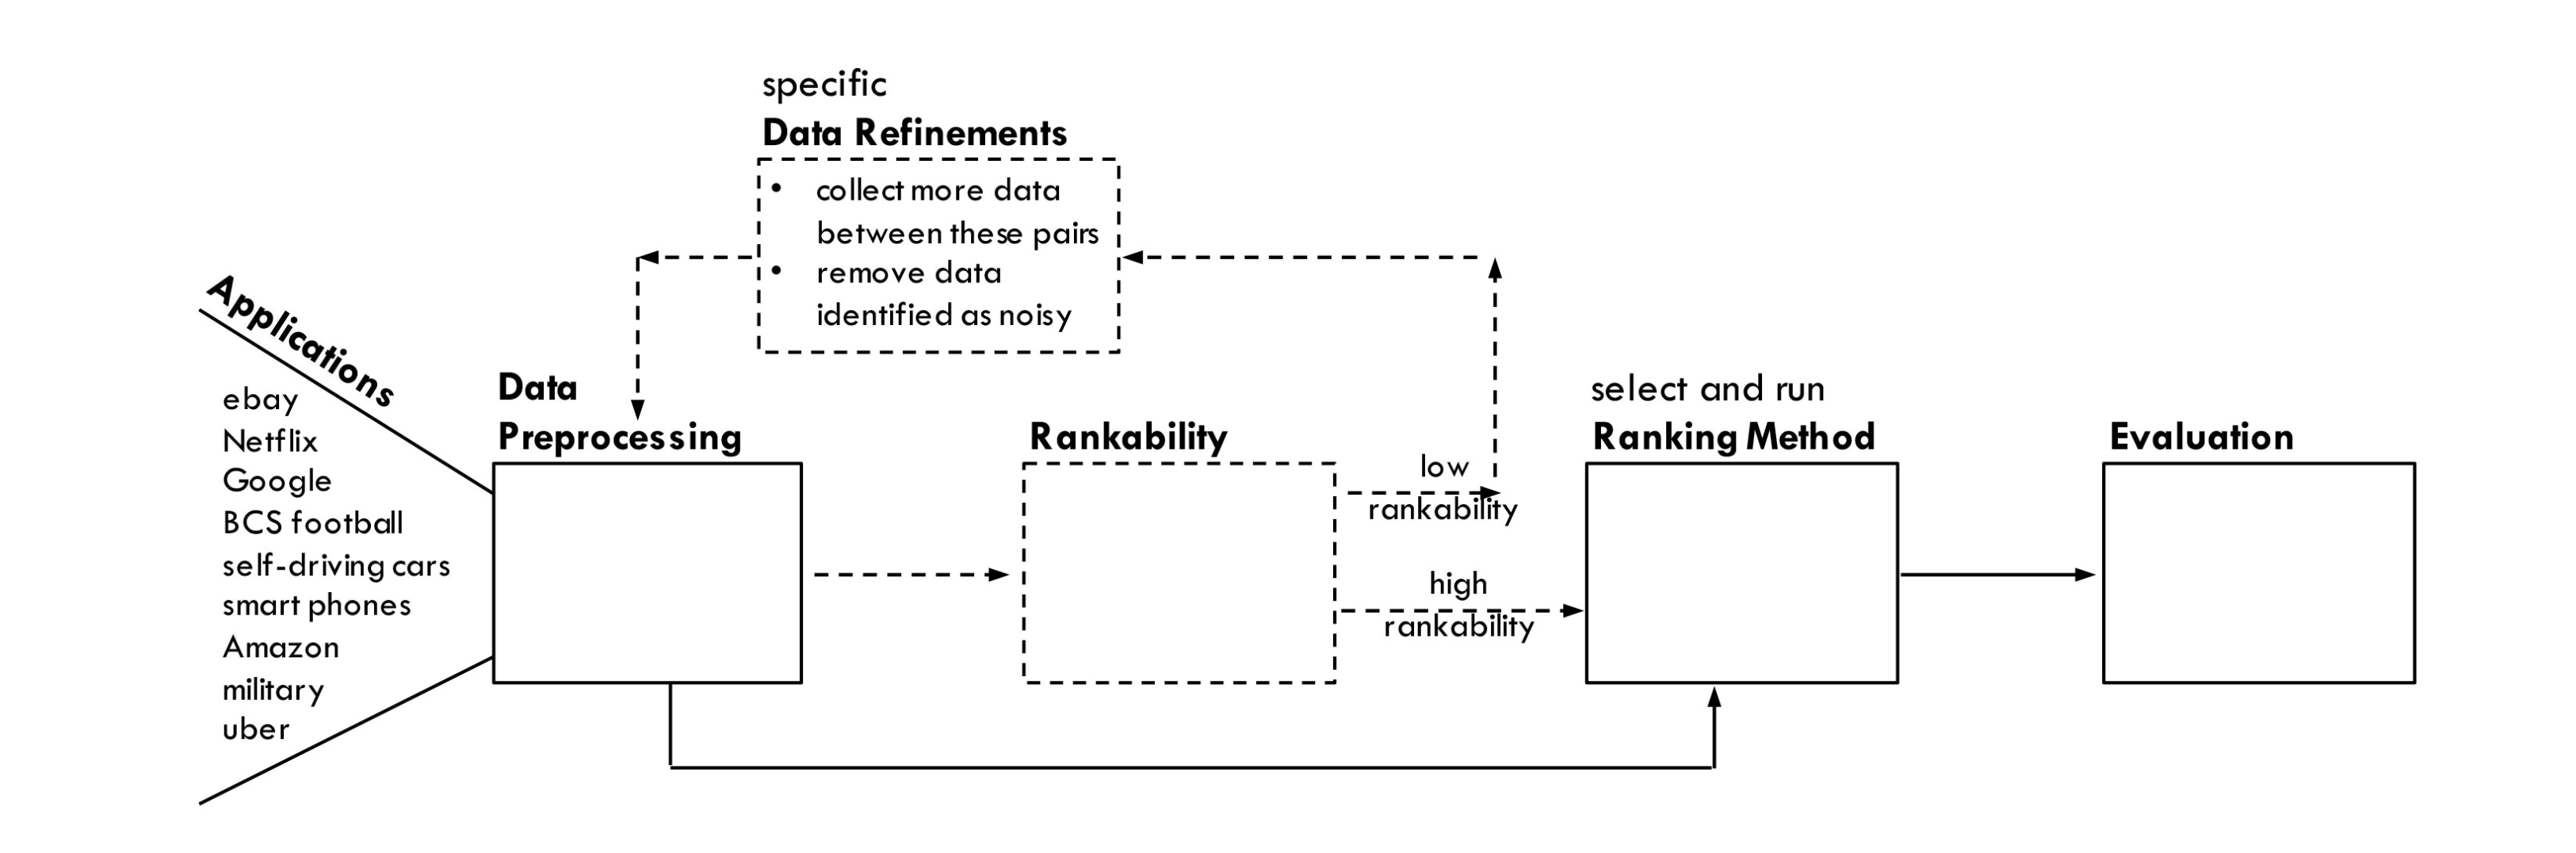
\includegraphics[width=.75\linewidth]{data_pipe}
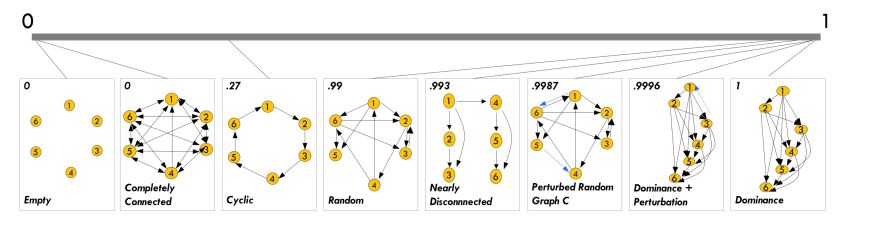
\includegraphics[width=.75\linewidth]{ranking}

\subsection{Why} The reason why I wanted to share this article is because there is often a black-box effect with online search and buzzwords tend to mystify subject in my own opinion. But, with a little intuition, anyone can begin to learn any subject and in this matter, the algorithm that people refer too is indeed abstract but the subjects used to implements ranking use rankibility calculation before evaluating if a result is approriate to share. This implementation can have geo-politicals. For instance, companies and even countries have been known to implement ranking toll that aides in making highstake descisions like brokering resolutions to conflicts in South Africa, Northern Ireland, and Israel-Palestine \autocite. I feel it is important to demystify current technologies because their effectts ripple through most facets of our lives and plus, I find it interesting to know how the algorithm is sort-of implemented even though I do not fully understand it. Making an attempt to understand a complex is better than making no attempt.

\printbibliography

\end{document}
